\documentclass[dvisvgm,tikz,border=4pt]{standalone}
\usepackage{amsmath,amssymb}

\usetikzlibrary{arrows.meta,positioning,automata,shapes,shapes.misc,calc,decorations.pathmorphing,decorations.markings,angles,quotes,patterns,mindmap,matrix,knots,hobby,trees}
\tikzset{->-/.style={decoration={markings, mark=at position 0.5 with {\arrow{Stealth}}}, postaction={decorate}}}
\begin{document}
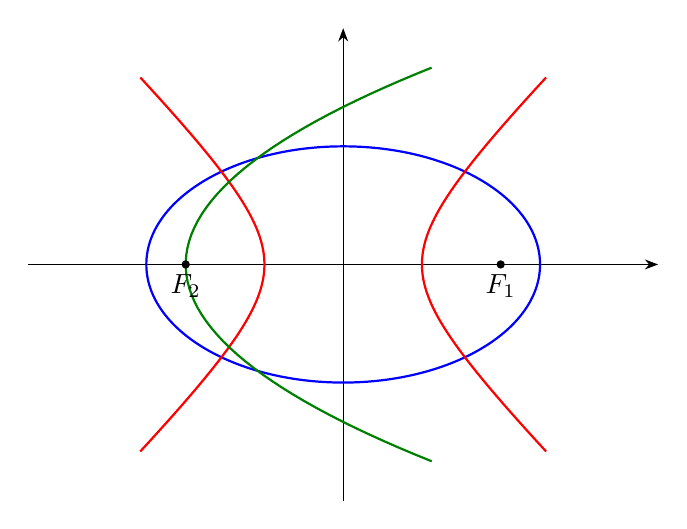
\begin{tikzpicture}[>=Stealth]
\draw[->] (-4,0) -- (4,0); \draw[->] (0,-3) -- (0,3);
\draw[thick, blue] (0,0) ellipse (2.5 and 1.5);
\draw[thick, red, domain=-1.6:1.6, samples=60] plot ({cosh(\x)}, {sinh(\x)});
\draw[thick, red, domain=-1.6:1.6, samples=60] plot ({-cosh(\x)}, {sinh(\x)});
\draw[thick, green!50!black, domain=-2.5:2.5, samples=60] plot ({\x*\x/2-2}, {\x});
\fill (2,0) circle (1.5pt) node[below] {$F_1$}; \fill (-2,0) circle (1.5pt) node[below] {$F_2$};
\end{tikzpicture}
\end{document}
